\chapter{Metodologia Proposta}
\label{chap3}

No capítulo anterior, foram apresentados os conceitos e as tecnologias relevantes para a compreensão da solução de monitoramento desenvolvida. Contudo, vale ressaltar que nem todas as ferramentas descritas anteriormente foram efetivamente empregadas na implementação final da proposta.

Este capítulo tem por objetivo detalhar todo o processo de desenvolvimento da solução de monitoramento, desde as primeiras considerações e escolhas de arquitetura, passando pela seleção e adaptação das ferramentas adotadas, até a apresentação da solução final implementada. Serão discutidas as motivações para determinadas decisões técnicas, desafios encontrados ao longo do desenvolvimento, e os métodos empregados para contorná-los, buscando sempre respaldar as opções feitas com base nos conceitos apresentados no Capítulo 2. Também são descritos os equipamentos utilizados durante o desenvolvimento e todo o código fonte do projeto está versionado no repositório Git \citep{vitorcossetti2025}.

As especificações do sistema operacional serão apresentadas posteriormente, visto que a escolha desse aspecto evoluiu ao longo do desenvolvimento, conforme será detalhado neste capítulo.

\section{Abordagem Preliminar}
\label{section:AbordagemPreliminar}

Esta seção apresenta uma visão geral das decisões iniciais tomadas antes da definição da arquitetura final da solução de monitoramento. As primeiras etapas deste trabalho podem ser divididas em dois momentos: inicialmente, o escopo era voltado para o monitoramento de infraestruturas de TI tradicionais (como servidores e clusters); em seguida, evoluiu para englobar também dispositivos conectados à rede de forma abrangente, sem restrições de tipagem.

\subsection{Escopo inicial - Infraestrutura Tradicional}
\label{subsection:EscopoInicial}

Durante as discussões preliminares, o objetivo era monitorar servidores. Foi considerada uma arquitetura onde um dispositivo -- podendo ser um NUC ou Raspberry Pi com softwares instalados -- realizaria a coleta de métricas deste servidor e, após o processamento destes dados, disponibilizaria-os em painéis com visualizações gráficas especializadas. Alternativas com Orange Pi como equipamento foram analisadas, mas a escolha final recaiu sobre o NUC ou Raspberry Pi devido à suas respectivas popularidades e suporte.

Entretanto, como não foi possível adquirir fisicamente um NUC ou Raspberry Pi, decidiu-se simular toda a \foreign{stack} de monitoramento em uma máquina virtual. Com isso, a possibilidade da utilização de distribuições ou versões do Raspberry Pi OS para fins de desenvolvimento foi descartada, por tratar-se de um sistema operacional baseado em arquitetura ARM, incompatível com a arquitetura x86-64 dos equipamentos disponíveis.

No desktop disponível, à época com sistema operacional não-Linux, instalou-se o VMWare Workstation Player (versão gratuita do VMWare Workstation) para configuração de uma VM com Rocky Linux. A escolha pelo Rocky Linux baseou-se em sua compatibilidade com o CentOS, estabilidade e longo ciclo de suporte, características valorizadas em ambientes corporativos.

No entanto, o VMWare Workstation Player mostrou-se limitado em recursos, dificultando a execução de múltiplas VMs. Por isso, migrou-se para o VirtualBox, o que trouxe maior flexibilidade e controle.

Esta estratégia inicial apresentou limitações importantes: a primeira era a maior dificuldade na aquisição de dados, pois seria necessário obter um servidor físico para coleta dos mesmos. Outra limitação foi o elevado custo computacional inerente ao uso de VMs em comparação a soluções baseadas em contêineres, e pouca modularidade, resultando em manutenção complexa e baixa praticidade.

Devido a esses fatores, verificou-se a necessidade de reavaliar o escopo e buscar abordagens mais aderentes aos recursos disponíveis e aos objetivos do projeto.

\begin{figure}[H]
\centering
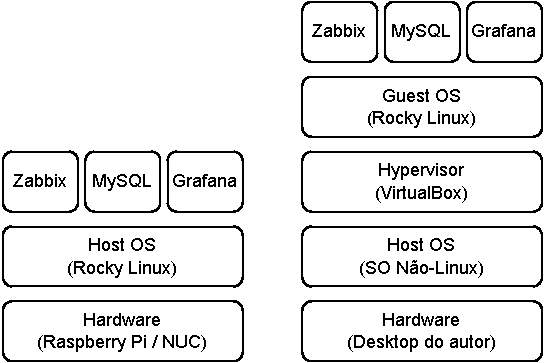
\includegraphics[scale=1]{Imagens/chap03/v0xv1_stack.pdf}
\caption{\textcolor{red}{Da esquerda para a direita - \foreign{stack} conceitual, \foreign{stack} implementada.}}
\label{fig:StackImplementada}
\end{figure}

\begin{figure}[H]
\centering
\setlength{\abovecaptionskip}{-20pt}
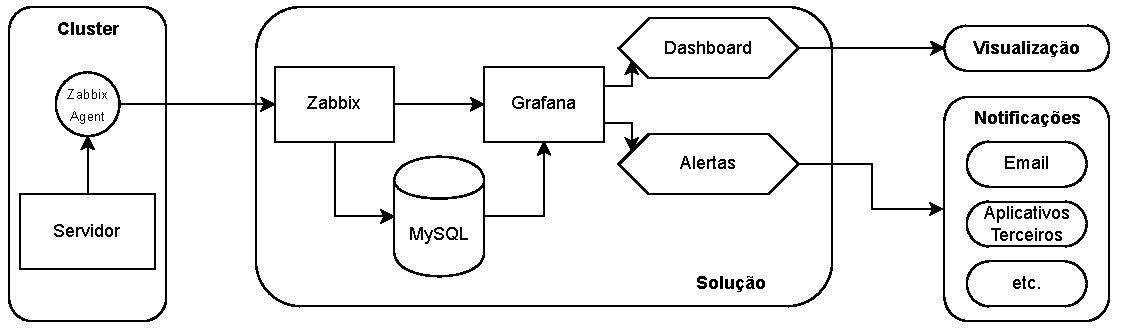
\includegraphics[width=\textwidth]{Imagens/chap03/v0_diagram.pdf}
\caption{\textcolor{red}{Arquitetura conceitual.}}
\label{fig:ArquiteturaConceitual}
\end{figure}

\begin{figure}[H]
\centering
\setlength{\abovecaptionskip}{-20pt}
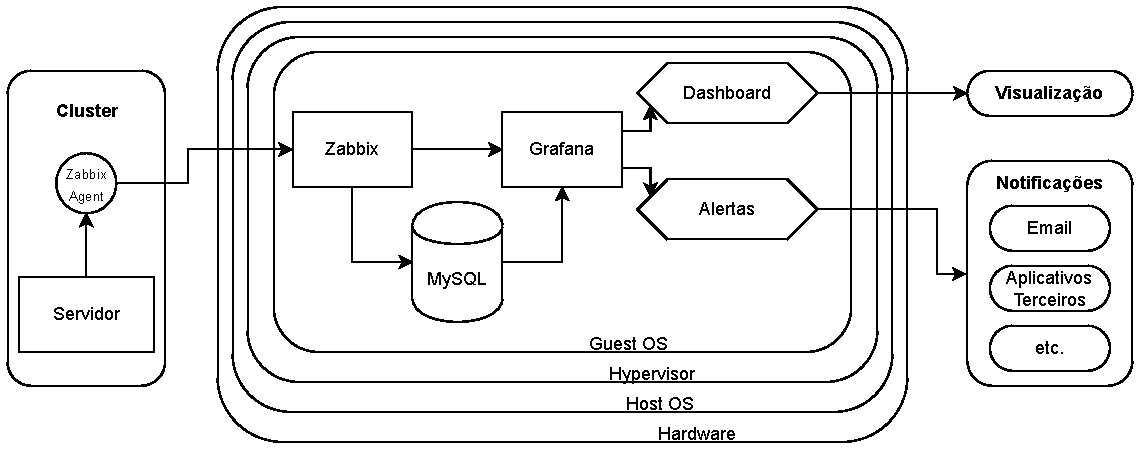
\includegraphics[width=\textwidth]{Imagens/chap03/v1_diagram.pdf}
\caption{\textcolor{red}{Arquitetura implementada.}}
\label{fig:ArquiteturaImplementada}
\end{figure}

\subsection{Escopo Reformulado - Monitoramento Amplo}
\label{subsection:EscopoReformulado}

Até então, os sistemas operacionais dos \foreign{hosts} disponíveis eram distintos (o desktop com um sistema não-Linux e o notebook com Ubuntu Desktop). Considerando as limitações encontradas na abordagem inicial, optou-se por instalar o Ubuntu Server no desktop como SO\abbrev{SO}{Sistema Operacional} para experimentação.

Conforme relatado na literatura, o Ubuntu Server demonstrou desempenho satisfatório e baixo consumo de recursos. Contudo, havia dois equipamentos sendo utilizados no desenvolvimento do projeto: 1 -- desktop do próprio autor, sem qualquer restrição para troca e alteração de hardware e software; 2 -- notebook corporativo em que o sistema operacional não poderia ser alterado. Visando padronizar os ambientes de desenvolvimento, decidiu-se por padronizar o SO no Ubuntu Desktop em ambos os dispositivos.

No decorrer dessas alterações, a abordagem de monitoramento foi ampliada para contemplar não apenas servidores, mas também uma ampla variedade de dispositivos conectados à rede. Essa redefinição proporcionou maior versatilidade ao projeto, tornando desnecessária a aquisição de servidores físicos e possibilitando a utilização de contêineres tanto para a simulação de dispositivos quanto para a implementação da \foreign{stack} de monitoramento. Com isso, o processo de desenvolvimento tornou-se mais prático, ágil e modular, além de permitir um aproveitamento mais eficiente dos recursos computacionais disponíveis. Cabe destacar ainda que, ao adotar contêineres não só para testes, mas também para toda a infraestrutura de monitoramento, a discussão sobre a necessidade de hardware específico, como NUC ou Raspberry Pi, perdeu relevância neste contexto, já que a solução desenvolvida pode ser executada em qualquer máquina compatível com tecnologias de conteinerização.

%TODO: Em trabalhos futuros a análise de viabilidade de implementação em NUC ou Raspberry Pi
\begin{figure}[H]
\centering
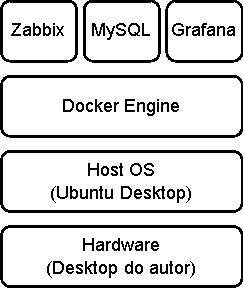
\includegraphics[scale=0.96]{Imagens/chap03/v2_stack.pdf}
\caption{\textcolor{red}{\foreign{Stack} reformulada.}}
\label{fig:StackReformulada}
\end{figure}

\begin{figure}[H]
\centering
\setlength{\abovecaptionskip}{-20pt}
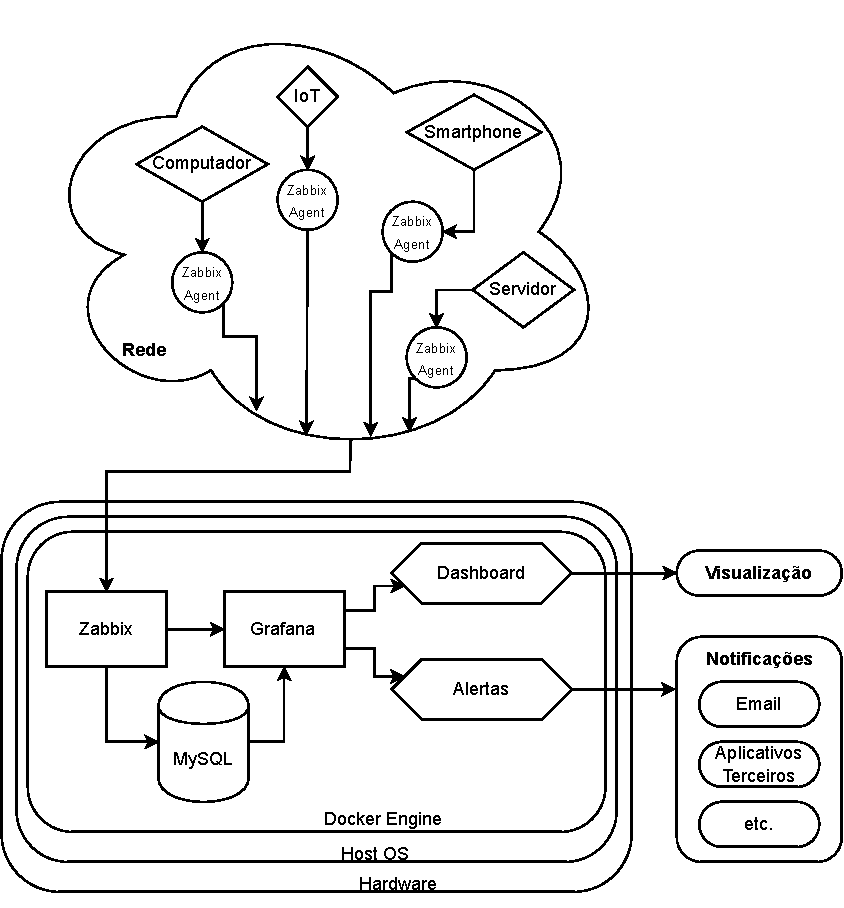
\includegraphics[width=\textwidth]{Imagens/chap03/v2_diagram.pdf}
\caption{\textcolor{red}{Arquitetura reformulada.}}
\label{fig:ArquiteturaReformulada}
\end{figure}


\subsection{Das versões iniciais}
\label{subsection:VersõesIniciais}

A virtualização desempenha um papel essencial neste trabalho. Além dos benefícios já mencionados, a conteinerização utilizando orquestradores como Docker Compose permite o versionamento de todo o trabalho desenvolvido em repositórios de controle de versão, como o Git. Esta abordagem rege todo o trabalho a seguir.

Desde o início do projeto, o Zabbix foi escolhido como principal ferramenta de monitoramento. Mesmo após a reformulação do escopo, o Zabbix permaneceu como a solução central, devido à sua capacidade de atender todos os requisitos do projeto: possui interface web, é de código aberto, é amplamente utilizado e consolidado no mercado, sendo compatível com diversos sistemas operacionais, arquiteturas e possuindo ampla documentação e ferramentas como agentes, proxies e servidores. Além disso, o Zabbix é altamente escalável, permitindo a adição de novos dispositivos e serviços monitorados de forma simples e eficiente.

Tendo o Zabbix como sistema de monitoramento central, posteriormente aco\-plaria-se a ele o Grafana. Apesar do Zabbix já possuir uma interface web com \foreign{dashboards} e gráficos, o Grafana oferece uma experiência de visualização mais rica e personalizável, sendo um complemento ideal.

A partir do repositório Docker oficial do Zabbix  \citep{zabbixdocker2025}, fez-se um \foreign{fork} para o repositório dedicado a este projeto. Essa abordagem permitiu a experimentação com os principais recursos conteinerizados da ferramenta, como servidor Zabbix, banco de dados MySQL, e agentes. O servidor foi inicialmente configurado com um \foreign{dashboard} básico, aproveitando o modelo fornecido pelo repositório Zabbix-Docker.

Após a execução bem-sucedida dos contêineres que compunham o sistema de monitoramento central, procedeu-se à instalação de um agente Zabbix no dispositivo móvel do autor para fins de teste. Foi possível realizar o \foreign{ping} do dispositivo a partir do servidor, sendo ambos — o agente conteinerizado e o instalado no dispositivo móvel — devidamente adicionados à lista de \foreign{hosts} do servidor.

É importante ressaltar que o Zabbix não dispõe de agentes oficiais para dispositivos móveis, mas disponibiliza recomendações de versões não oficiais desenvolvidas por terceiros para esse tipo de aplicação.

Durante essas implementações, foram identificados alguns pontos críticos que impactaram a continuidade do Zabbix como ferramenta principal de monitoramento do projeto: a necessidade de executar um contêiner adicional exclusivamente para o banco de dados (MySQL ou Postgres) eleva o custo computacional do ambiente; a interface gráfica do Zabbix apresentou limitações quanto à navegabilidade e usabilidade, dificultando a adaptação do autor; e o projeto Zabbix-Docker, por abranger múltiplas configurações, mostrou-se extenso e complexo, o que dificultou a leitura, compreensão e manutenção do código.

Além desses aspectos, o autor enfrentava simultaneamente a curva de aprendizado do Zabbix e do Docker, o que elevou significativamente o esforço necessário para a evolução do projeto. Tal cenário levou à decisão de abandonar o Zabbix, optando-se pela adoção do Prometheus nas etapas subsequentes deste trabalho.

\begin{figure}[H]
\centering
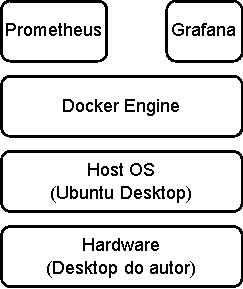
\includegraphics[scale=1]{Imagens/chap03/v3_stack.pdf}
\caption{\textcolor{red}{\foreign{Stack} da versão base do projeto.}}
\label{fig:StackBase}
\end{figure}
\begin{figure}[H]
\centering
\setlength{\abovecaptionskip}{-20pt}
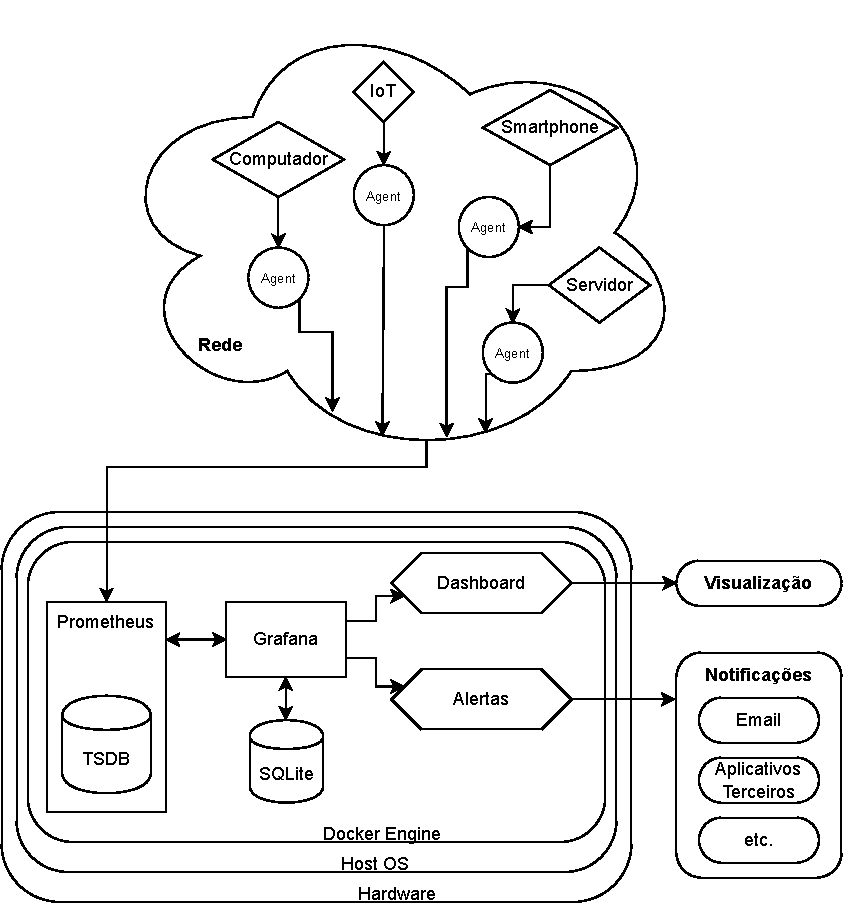
\includegraphics[width=\textwidth]{Imagens/chap03/v3_diagram.pdf}
\caption{\textcolor{red}{Arquitetura da versão base do projeto.}}
\label{fig:ArquiteturaBase}
\end{figure}

\section{Descrição da Arquitetura da Solução}

Placeholder

---é aqui que irei descrever toda a minha jornada de implementação---

\section{Infraestrutura}

Placeholder


Foram utilizados dois computadores, cujas especificações são apresentadas na Tabela \ref{tab:available-hardware}.

\begin{table}[H]
\centering
\caption{Especificações de hardware dos equipamentos disponíveis}
\label{tab:available-hardware}
\begin{tabular}{lcc}
\toprule
\textbf{Componente} & \textbf{Desktop} & \textbf{Notebook} \\
\midrule
CPU   & Intel Core i5-7600   & Intel Core i7-8565U \\
RAM   & 16GB                 & 32GB                \\
Disco & 500GB (SSD)            & 250GB (SSD)          \\
\bottomrule
\end{tabular}
\end{table}



\section{Discussão sobre as métricas}

Placeholder

\section{Aplicação de Monitoramento}

Placeholder

Falar dos alertas e notificações
Discorrer sobre o dashboard em si